\documentclass[conference]{IEEEtran}
\IEEEoverridecommandlockouts
% The preceding line is only needed to identify funding in the first footnote. If that is unneeded, please comment it out.
\usepackage{cite}
\usepackage{amsmath,amssymb,amsfonts}
\usepackage{graphicx}
\usepackage{textcomp}
\usepackage{url}
\usepackage{xcolor}
\def\BibTeX{{\rm B\kern-.05em{\sc i\kern-.025em b}\kern-.08em
T\kern-.1667em\lower.7ex\hbox{E}\kern-.125emX}}
\begin{document}

% Custom commands:
  \newcommand{\coo}{\ensuremath{\mathrm{CO_2}}}

% -----------------------------------
% -------------- TITLE --------------
\title{RoadAI - A Multiagent Reinforcement Learning Approach to Reducing \coo{} Emissions at a Construction Site}
% -----------------------------------



% -----------------------------------
% ------------- AUTHORS -------------
% -----------------------------------
\author{
	\IEEEauthorblockN{Viktor Ringvold Hasle}
	\IEEEauthorblockA{\textit{Dept. of Informatics} \\
	\textit{University of Oslo}\\
	Oslo, Norway \\
	viktorrh@ifi.uio.no}
	\and
	\IEEEauthorblockN{Ada Hatland}
	\IEEEauthorblockA{\textit{Dept. of Informatics} \\
	\textit{University of Oslo}\\
	Oslo, Norway \\
	adaha@ifi.uio.no
	}
	\and
	\IEEEauthorblockN{Elias Lynum Ringkjøb}
	\IEEEauthorblockA{\textit{Dept. of Informatics} \\
	\textit{University of Oslo}\\
	Oslo, Norway \\
	eliaslr@ifi.uio.no
	}
	\and
	\IEEEauthorblockN{Ilya Berezin}
	\IEEEauthorblockA{\textit{Dept. of Informatics} \\
	\textit{University of Oslo}\\
	Oslo, Norway \\
	ilyab@ifi.uio.no}
	\and \\
	\IEEEauthorblockN{Tom Frode Hansen}
	\IEEEauthorblockA{\textit{NGI- Norges Geotekniske Institutt} \\
	Oslo, Norway \\
	tom.frode.hansen@ngi.no
	}
}

  \maketitle


  % -----------------------------------
  % ------------ ABSTRACT -------------
  % -----------------------------------
  % \begin{abstract}
  % % Abstract is last thing we should write.

  % % Should have 3-5 keywords.
  % Index Terms - Multi-Agent Reinforcement Learning (MARL),
  % \end{abstract}


  % -----------------------------------
  % ---------- INTRODUCTION  ----------
  % -----------------------------------
  \section{Introduction}
  Carbon dioxide (\coo{}) emission is one of the largest contributions to greenhouse gasses and global warming.
  Reducing \coo{} emissions is an important step in preventing global warming and all of the negative
  consequences associated with it. Norway's total greenhouse gas emissions were, according to Statistics
  Norway, in 2022 48.9 million tonnes of \coo{}
  equivalences\footnote{https://www.ssb.no/natur-og-miljo/forurensning-og-klima/statistikk/utslipp-til-luft}.
  1.5\% of which are emitted by construction machines. \cite{noraRoadAIReducing} The reduction of such
  a significant percentage of the total emissions is a crucial task.

  This project is based on the RoadAI competition held by Norwegian Artificial Intelligence Research
  Consortium (NORA). \cite{noraRoadAIReducing} The objective in the RoadAI competition is to reduce the
  total \coo{} emissions from a road construction site using machine learning methods.In this paper, we will
  present a method for using Multiagent Reinforcement Learning (MARL) algorithms in order to reduce such
  emissions.

  % RL for GHG reduction
  In a study from 2022, a group of researchers from Germany and Switzerland used reinforcement learning
  (RL) for route optimization of marine transport. \cite{MORADI2022111882} This study ... \textless Elaborate. You need
  Eduroam to read the article\footnote{\url{https://www.sciencedirect.com/science/article/abs/pii/S0029801822012239?casa_token=kkxSoukxDkgAAAAA:eDAPRTWeGqMvCvfZxtBB9mJLswCbGDP2922zGX3HWtWn_hDtYkWM_PWqaJWsSmJBTc42HzL8BYI}} \textgreater

  Another study from Canada \cite{HUO2023106664} showed promising results in reduction of greenhouse gas
  emissions
  from dump trucks' fuel consumption in a open-pit mining fleet. This model is a Q-learning RL algorithm
  which aims to improve fleet productivity, and decreasing idle time, which in turn reduces the greenhouse
  gas emissions. It does so by offering a real-time, reactive,  dispatching system, rather than a manual
  fixed one. The RL model, trained on a simulated environment, takes into account traffic, queueing,
  payload and maintenence requirements. As a result, the model showed an up to 30\% reduction in greenhouse
  gases while having no impact on production levels.

  % MARL

  % Environments

  % PPO / MAPPO

  % DQN / QMIX

	% -----------------------------------
	% ------------- METHODS -------------
	% -----------------------------------
	\section{Methodology}

	The goal of the Road AI project is to demonstrate an algorithm that could reduce emissions from road construction.
	We are using MARL to train agents on a simulation of road construction and to demonstrate how it can be utilized to solve this problem.
	Our methodology primarily focuses on the utilization of Multi-Agent Reinforcement Learning to tackle the problem of emissions in road construction. Given the complexity of the task, we adopted a step-by-step approach to ensure that the model is not only accurate but also efficient.

	\subsection{Problem Formulation}
	The first step in our methodology was to formulate the problem in the context of MARL. We defined each construction vehicle as an agent with its own set of actions, observations, and rewards. The joint action space consisted of moving, idling, loading, or unloading materials. Observations for each agent included the status of the road construction, the position of other agents, and the current load of materials. Rewards were also implemented to promote actions that lead to reduced emissions.

	\subsection{Simulation Environment}
	To train our agents, we developed a custom simulation environment using the PettingZoo framework. The environment replicates a typical road construction site, with details like topography and material locations. In this environment every object is represented as a particle in a grid.
	The agents of the simulation, construction trucks are able to move cardinally in this grid with the goal of hauling construction materials from excavators to the unfinished road.
	Every agent gets assigned a reward for each action they take with positive rewards for productive moves, and negative rewards for unproductive ones (idling, or unnecessary moving).

	While simulating the trucks we collect the rewards which the reinforcement learning algorithms uses to train.
	Using the average episodic rewards we can estimate the algorithms performance over the training, and compare them to eachother.
	\begin{figure}
		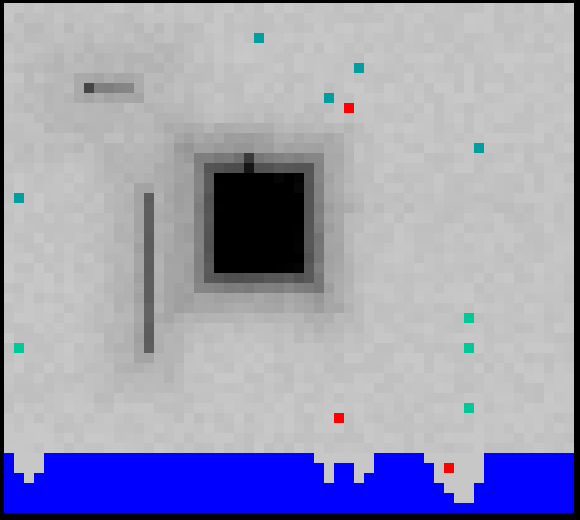
\includegraphics[width=0.9\columnwidth]{graphs/example_env.png}
		\caption{Example randomly generated environment}
	\end{figure}
	While this environment is very simplified in contrast to real life, it easy to randomly generate and lightweight.

	\subsection{MAPPO}
	We used the Stable-baselines implementation of the PPO algorithm to train our agents.
	PPO works by gradient ascent to find the optimal policy, and has been shown to produce good results in similiar cooperative environments. % INSERT SITATION HERE
    PPO is an actor-critic method that is currently considered state of the art. 
    It implements clipping of the gradient to ensure we don't overshoot when climbing. 
    It is also stochastic by design where the policy $\pi_\theta$ chooses random actions according to a certain heat which decreases over time. 

	\subsection{Multiagent DQN}
    We attempted a version of DQN where the reward for an action is given as the average reward for all the actions in that timestep. The issue with this is that it might reward a "bad" action and punish a "good" action if the average reward that timestep was high or low respectively, it turns out not treating it as a cooperative system but rather a system where every agent attempts to maximise their own reward is significantly more effecient. It's possible that with better hyperparameters or longer training time our multi agent implementation of DQN might outperform the single agent implementation, but with the training time and hyperparameters used we struggled to get positive rewards at all with this approach. We ended up using StableBaselines implementation of DQN.
	\subsection{Stable-baselines}
	While stable-baselines is not inherently compatible with multi-agent environments we found that if you
	make it so that each agent steps

	\subsection{Training Procedure}
	Each algorithm was trained for 250 episiodes of a fixed length of 5000 steps. In total the training was 1250000 timesteps and took about 2 hours on a gpu.

	\subsection{Evaluation}
	Post-training, we evaluated our models based on following metrics:
	\begin{enumerate}
		\item Mean episodic reward
		\item Number of road pieces built per step
	\end{enumerate}

	\begin{figure}[h!]
		%TODO ADD new image
		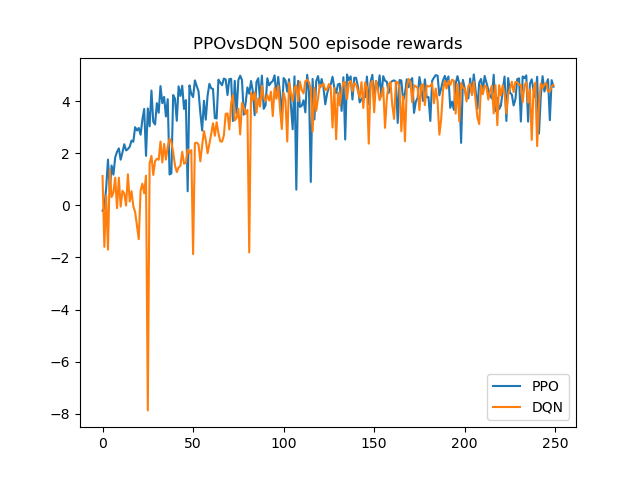
\includegraphics[width=\columnwidth]{graphs/PPOvsDQN250.png}
		\caption{Mean Episodic rewards}
	\end{figure}

	As you could see from the graphs the algorithms performed quite similiarly.

	\subsection{Hyperparameter Optimization}
	We used the optuna library to hyperparameter optimize our the PPO algorithm. Optuna uses a baynesian search to find the best parameters for us. This way we could make sure that our results


	% -----------------------------------
	% ------ RESULTS AND DISCUSSION -----
	% -----------------------------------


	% -----------------------------------
	% ---------- RELATED WORK -----------
	% -----------------------------------
	\section{Related works}
	SMACv2\cite{ellis2022smacv2} evaluates two MARL algorithms for problems using centralized training with
	decentralized execution (CTDE); QMIX and MAPPO.

	QMIX employs a centralized critic to estimate joint action-value functions, while MAPPO uses a decentralized
	actor-critic framework with a centralized value function.

	QMIX outperformed MAPPO on most scenarios, but QMIX is memory-intensive due to its large replay buffer. For
	this reason, QMIX requires more computational power. In addition, the paper notes that MAPPO was still
	increasing its performance at the time of termination in several scenarios, which indicates it could end up
	with a better result.

	This paper aims to evaluate both the QMIX and MAPPO algorithms.


	Flatlands\cite{laurent2021flatland} was a competition where contestants to design a MARL algorithm for
	train scheduling. This is similar to the approach we seek to use to solve RoadAI.
	In the competition MAPPO performed well and is a pointer for what we could use in our own MARL implementation.


	The application of Multi-Agent Reinforcement Learning (MARL) for carbon reduction in the construction industry is relatively recent field. Here are some other related works:

	\begin{itemize}

		\item \textbf{Optimized Resource Allocation:}
			MARL has been used to optimize resource allocation in construction sites, ensuring that machinery and equipment are used in a most efficient way. By minimizing idle times and optimizing machinery routes, fuel consumption can be reduced, leading to a decrease in carbon emissions\cite{resource_allocation}.

		\item \textbf{Dynamic Scheduling:}
			Construction projects often involve multiple tasks that need a proper coordination. MARL algorithms has been used for dynamic scheduling, ensuring that tasks are carried out in an optimized way, reducing potential delays and minimizing the carbon footprint due to inefficiencies\cite{dynamic_scheduling}.

	\end{itemize}

	While the above works have shown the potential of MARL, there is still potential to explore with the advent of newer algorithms. The main challenge remains in integrating these advanced techniques seamlessly into the traditional construction processes and ensuring real-world applicability.

	\noindent


	% -----------------------------------
	% ----------- CONCLUSION ------------
	% -----------------------------------
	\section{Conclusion}




% -----------------------------------
% ------------- METHODS -------------
% -----------------------------------
\section{Methodology}

The goal of the Road AI project is to demonstrate an algorithm that could reduce emissions from road construction.
We are using MARL to train agents on a simulation of road construction and to demonstrate how it can be utilized to solve this problem.
Our methodology primarily focuses on the utilization of Multi-Agent Reinforcement Learning to tackle the problem of emissions in road construction. Given the complexity of the task, we adopted a step-by-step approach to ensure that the model is not only accurate but also efficient.

\subsection{Problem Formulation}
The first step in our methodology was to formulate the problem in the context of MARL. We defined each construction vehicle as an agent with its own set of actions, observations, and rewards. The joint action space consisted of moving, idling, loading, or unloading materials. Observations for each agent included the status of the road construction, the position of other agents, and the current load of materials. Rewards were also implemented to promote actions that lead to reduced emissions.

\subsection{Simulation Environment}
To train our agents, we developed a custom simulation environment using the PettingZoo framework. The environment replicates a typical road construction site, with details like topography and material locations. In this environment every object is represented as a particle in a grid.
The agents of the simulation, construction trucks are able to move cardinally in this grid with the goal of hauling construction materials from excavators to the unfinished road.
Every agent gets assigned a reward for each action they take with positive rewards for productive moves, and negative rewards for unproductive ones (idling, or unnecessary moving).

While simulating the trucks we collect the rewards which the reinforcement learning algorithms uses to train.
Using the average episodic rewards we can estimate the algorithms performance over the training, and compare them to eachother.
\begin{figure}
  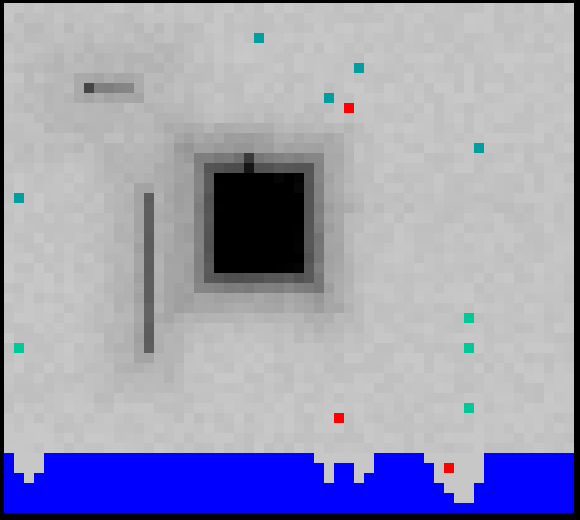
\includegraphics[width=0.9\columnwidth]{graphs/example_env.png}
  \caption{Example randomly generated environment}
\end{figure}
While this environment is very simplified in contrast to real life, it easy to randomly generate.

\subsection{MAPPO}
We used the Stable-baselines implementation of the PPO algorithm to train our agents.
PPO works by gradient ascent to find the optimal policy, and has been shown to produce good results in similiar cooperative environments. % INSERT SITATION HERE


\subsection{Multiagent DQN}

\subsection{Training Procedure}
Each algorithm was trained for 250 episiodes of a fixed length of 5000 steps. In total the training was 1250000 timesteps and took about 2 hours on a gpu.

\subsection{Evaluation}
Post-training, we evaluated our models based on following metrics:
\begin{enumerate}
  \item Mean episodic reward
  \item Number of road pieces built per step
\end{enumerate}

\begin{figure}[h!]
  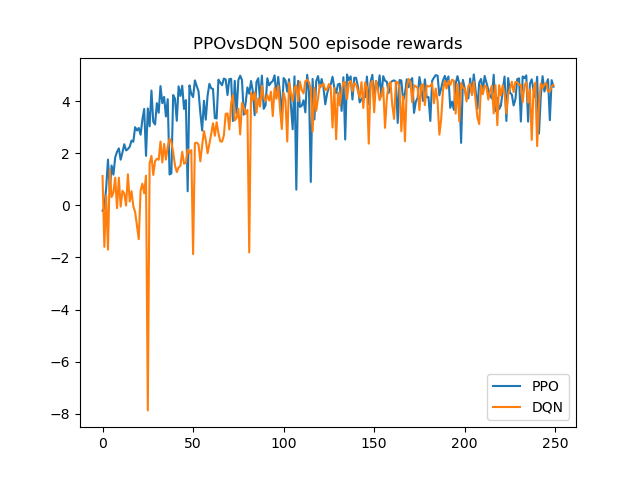
\includegraphics[width=\columnwidth]{graphs/PPOvsDQN250.png}
  \caption{Mean Episodic rewards}
\end{figure}

As you could see from the graphs the algorithms performed quite similiarly.

\subsection{Hyperparameter Optimization}
We used the optuna library to hyperparameter optimize our the PPO algorithm. Optuna uses a baynesian search to find the best parameters for us. This way we could make sure that our results


% -----------------------------------
% ------ RESULTS AND DISCUSSION -----
% -----------------------------------


% -----------------------------------
% ---------- RELATED WORK -----------
% -----------------------------------
\section{Related works}
SMACv2\cite{ellis2022smacv2} evaluates two MARL algorithms for problems using centralized training with
decentralized execution (CTDE); QMIX and MAPPO.

QMIX employs a centralized critic to estimate joint action-value functions, while MAPPO uses a decentralized
actor-critic framework with a centralized value function.

QMIX outperformed MAPPO on most scenarios, but QMIX is memory-intensive due to its large replay buffer. For
this reason, QMIX requires more computational power. In addition, the paper notes that MAPPO was still
increasing its performance at the time of termination in several scenarios, which indicates it could end up
with a better result.

This paper aims to evaluate both the QMIX and MAPPO algorithms.


Flatlands\cite{laurent2021flatland} was a competition where contestants to design a MARL algorithm for
train scheduling. This is similar to the approach we seek to use to solve RoadAI.
In the competition MAPPO performed well and is a pointer for what we could use in our own MARL implementation.


The application of Multi-Agent Reinforcement Learning (MARL) for carbon reduction in the construction industry is relatively recent field. Here are some other related works:

\begin{itemize}

  \item \textbf{Optimized Resource Allocation:}
    MARL has been used to optimize resource allocation in construction sites, ensuring that machinery and equipment are used in a most efficient way. By minimizing idle times and optimizing machinery routes, fuel consumption can be reduced, leading to a decrease in carbon emissions\cite{resource_allocation}.

  \item \textbf{Dynamic Scheduling:}
    Construction projects often involve multiple tasks that need a proper coordination. MARL algorithms has been used for dynamic scheduling, ensuring that tasks are carried out in an optimized way, reducing potential delays and minimizing the carbon footprint due to inefficiencies\cite{dynamic_scheduling}.

\end{itemize}

While the above works have shown the potential of MARL, there is still potential to explore with the advent of newer algorithms. The main challenge remains in integrating these advanced techniques seamlessly into the traditional construction processes and ensuring real-world applicability.

\noindent


% -----------------------------------
% ----------- CONCLUSION ------------
% -----------------------------------
\section{Conclusion}




% -----------------------------------
% ----------- REFERENCES ------------
% -----------------------------------
\newpage
% \nocite{*}        % This includes all references that haven't been explicitly cited
\bibliography{citations.bib}
\bibliographystyle{plain}


% -----------------------------------
% -------- ETHICS STATEMENT ---------
% -----------------------------------
\newpage

\appendices 
\section{Ethics Statement}
In the course of our project on Multiagent Reinforcement Learning, aimed at mitigating \coo{} emissions
from construction sites, we have conducted research that involves no experiments with human participants.
While this specific phase of our work does not directly raise concerns regarding wages or human
participation, it is essential to recognize that the technologies and methodologies we are developing
may eventually be applied in real-world settings where human interactions are integral. In such instances,
it becomes crucial to address ethical considerations associated with human safety and well-being.

We acknowledge that our current implementation serves as a simulation, and it is not as robust as a
real-world application would need to be. However, we are committed to exploring ways to ensure that the
agents, which are part of the system, incorporate safeguards to prevent harm to humans and machinery.
This commitment reflects our ethical responsibility to uphold the safety and welfare of individuals who
may interact with these agents in practical applications.

Moreover, our reinforcement learning framework includes a reward function that assigns a substantial
negative reward for agent collisions, with the intent of discouraging such incidents. The severity of
this negative feedback is designed to minimize the likelihood of agents crashing into one another. It
is important to note, though, that while our design minimizes such events, it does not guarantee their
complete avoidance.

The dataset we have employed for this project, generated by Skanska Norge AS and provided by Norwegian
Artificial Intelligence Research Consortium (NORA), does not contain any personally identifiable
information. Although the dataset's availability has yet to be confirmed, it was shared with us by NORA
following the conclusion of the RoadAI competition.

The primary objective of our project is to significantly reduce \coo{} emissions originating from
construction sites, potentially leading to substantial environmental and societal benefits.
Construction sites contribute 1.5\% of total Norwegian \coo{} emissions, making the reduction of
emissions in this sector a vital endeavour. Implementing our system across numerous construction sites
in Norway could result in a significant reduction in total \coo{} emissions, a crucial step toward a more
sustainable future.

In line with our commitment to ethical AI deployment, transparency and explainability need to be
addressed. It is imperative to ensure stakeholders can understand and trust the model's decisions.
Thus we have to make efforts to ensure that MARL algorithms are interpretable, allowing a comprehensive
understanding of factors influencing decisions.

Our research and project implementation do not support or enable any form of discrimination against
individuals or groups. Furthermore, they do not entail risks related to deception or harassment.
Our work is firmly rooted in legal activities and does not promote any restrictions on human rights.
Our ethical commitment is to conduct research and develop technologies that contribute to a greener,
more sustainable world without compromising the well-being of individuals or society as a whole.


\end{document}

% STRUCTURE:
% ----------

% Title - 1 sentence
%   (Your paper title should be specific, concise, and descriptive. Avoid using unnecessary words such as “new” or “novel”. Include keywords that will help a reader find your paper.)
%   Proposal: RoadAI - A Multiagent Reinforcement Learning approach to reducing \coo{} emissions at a construction site

% Abstract - 4 sentences
%   (Provide a concise summary of the research conducted. Include the conclusions reached and the potential implications of those conclusions. Your abstract should also:
%   - consist of a single paragraph up to 250 words, with correct grammar and unambiguous terminology;
%   - be self-contained with no abbreviations, footnotes, references, or mathematical equations;
%   - highlight what is unique in your work;
%   - include 3-5 keywords or phrases that describe the research, with any abbreviations clearly defined,  to help readers find your paper.)

% Introduction - 0.5-1 pages
%   (Help the reader understand why your research is important and what it is contributing to the field.
%   - Start by giving the reader a brief overview of the current state of research in your subject area.
%   - Progress to more detailed information on the specific topic of your research.
%   - End with a description of the exact question or hypothesis that your paper will address.
%   Also state your motivation for doing your research and what it will contribute to the field.)

% Methods - 2.5-3 pages
%   (Formulate your research question. It should include:
%   - a detailed description of the question;
%   - the methods you used to address the question;
%   - the definitions of any relevant terminology;
%   - any equations that contributed to your work.
%   The methods section should be described in enough detail for someone to replicate your work.)

%   Description of research question

%   Environment

%   PPO

%   DQN

% Results and Discussion - 0.5-1 page
%   (Show the results that you achieved in your work and offer an interpretation of those results. Acknowledge any limitations of your work and avoid exaggerating the importance of the results.)

% Related Work - 1.5-2 pages
%   (Related work)

% Conclusion - 1 page
%   (Summarize your key findings. Include important conclusions that can be drawn and further implications for the field.)

%   Future work
%     (Discuss benefits or shortcomings of your work and suggest future areas for research.)

% Acknowledgements - ????
%   (You can recognize individuals who provided assistance with your work, but who do not meet the definition of authorship. The acknowledgments section is optional.)

% References
